\documentclass[aspectratio=169]{beamer}
\usepackage[T1]{fontenc}
\usepackage[default]{sourcesanspro}
\usepackage{newtxsf}
\usepackage{hyperref}
\usepackage{latexsym,amsmath,xcolor,multicol,booktabs,calligra}
\usepackage{graphicx,pstricks,listings,stackengine}
\graphicspath{{./figures/}}
\usepackage{lipsum}
\usepackage{wrapfig}
\usepackage{url}
\usepackage{subcaption}
\usepackage{listings}
\usepackage{minted}
\setminted{fontsize=\footnotesize}
\usepackage{fontawesome5}

\usepackage{etoolbox}

\author{Yan Lin}
\title{AI Systems \& Infrastructure}
\subtitle{Module B.5: Edge Deployment}
\institute{%
    \href{https://www.yanlincs.com}{www.yanlincs.com}
}
\date{September 1st, 2026}
\usepackage{AAU}
\AtBeginSubsection{}
\setbeamertemplate{navigation symbols}{}
\ifdefined\hidenotes\else
    \setbeameroption{show notes on second screen=right}
    \setbeamerfont{note page}{size=\large}
    \hypersetup{pdfkeywords={SP-Right}}
\fi

\def\cmd#1{\texttt{\color{red}\footnotesize $\backslash$#1}}
\def\env#1{\texttt{\color{blue}\footnotesize #1}}
\definecolor{aauyellow}{RGB}{167, 131, 55}
\definecolor{aaublue}{RGB}{32, 26, 78}
\definecolor{aaured}{RGB}{152, 43, 28}
\definecolor{textgrey}{RGB}{60, 60, 60}

\setbeamercolor{normal text}{fg=textgrey}
\usebeamercolor[fg]{normal text}

\def\emphasis#1{{\color{aaured}\textbf{#1}}}
\def\live#1{{\color{aaublue}\textbf{Live demo:}} #1}
\renewcommand{\thefootnote}{}


\lstset{%
    basicstyle=\ttfamily\small,
    keywordstyle=\bfseries\color{deepblue},
    emphstyle=\ttfamily\color{deepred},
    stringstyle=\color{deepgreen},
    numbers=left,
    numberstyle=\small\color{halfgray},
    rulesepcolor=\color{red!20!green!20!blue!20},
    frame=shadowbox,
}

\begin{document}

\begin{frame}[plain,noframenumbering]
    \titlepage
    \vspace*{-0.6cm}
    \begin{figure}[htpb]
        \begin{center}
            
\includegraphics[keepaspectratio, scale=0.5]{aau-logo-left-uk}
        \end{center}
    \end{figure}
\note{
}
\end{frame}


\begin{frame}
\tableofcontents[sectionstyle=show,
subsectionstyle=show/shaded/hide,
subsubsectionstyle=show/shaded/hide]
\note{
}
\end{frame}



\section{When the Cloud Is Not the Right Answer}

\begin{frame}{Recap: where we are}
    In Module B.4 we deployed our AI server on a small cloud VM, gave it a domain name and an HTTPS certificate, and ended up with a real public AI service backed by infrastructure we did not have to own.

    \vspace{0.5em}
    Yet there are scenarios where running on a computer we have physical access to fits better than renting cloud capacity.
    \begin{itemize}
        \item A smart camera that has to react in milliseconds, where a cloud round trip is too slow
        \item An app processing medical scans we are not allowed to send to a third party
        \item A long-running service where the cumulative cloud bill has crossed the price of just buying a small server
    \end{itemize}
\note{
}
\end{frame}


\begin{frame}{Two related ideas}
    \begin{block}{Edge computing}
        Runs computation near where data is generated or where users interact with the system, instead of in a faraway data center.
        Motivated by \emphasis{where} data and users are.
    \end{block}

    \begin{block}{Self-hosting}
        Runs services on hardware we own and control, instead of renting capacity from a cloud provider.
        Motivated by \emphasis{who} owns the hardware.
    \end{block}

    \vspace{0.3em}
    Different concepts that come from different motivations, but they often overlap.
    A Raspberry Pi on our desk is both.
\note{
}
\end{frame}



\section{Edge and Self-Hosting}

\begin{frame}{Edge in the wild}
    The edge is the boundary of the network, where data first appears or where a person hits a button.

    \begin{itemize}
        \item A surveillance camera detecting someone at the door
        \item A self-driving car deciding whether to brake
        \item A smartphone running on-device speech recognition
    \end{itemize}

    \begin{block}{Why AI fits the edge}
        \begin{itemize}
            \item Latency drops, since the round trip to a data center disappears
            \item Bandwidth use drops, since not much data travels back to the cloud
            \item Privacy improves, since sensitive data never leaves the device
            \item The system keeps working when the internet goes down
        \end{itemize}
    \end{block}
\note{
}
\end{frame}


\begin{frame}{Self-hosting in the wild}
    By definition we have been self-hosting throughout this course.
    Every time we ran our AI server on our laptop, that was a self-hosted service.

    \begin{figure}[htpb]
        \begin{center}
            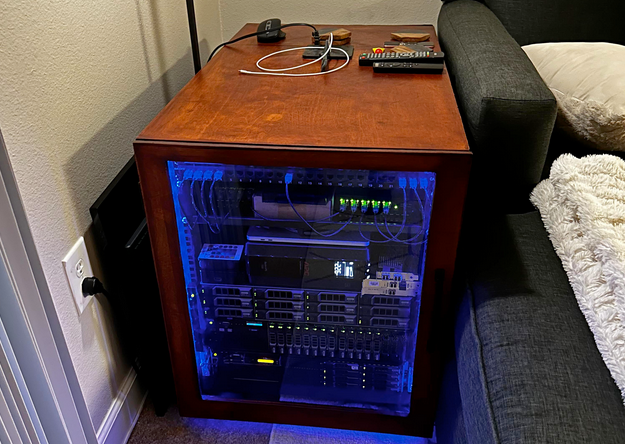
\includegraphics[width=0.3\textwidth]{diy_server_build}
        \end{center}
    \end{figure}

    The only difference vs a real self-hosted setup is that we did not put the laptop on a shelf and leave it running 24/7.

    The motivation is mostly the inverse of the cloud's selling points: ownership of the hardware, control over data, predictable cost, no vendor lock-in.
\note{
}
\end{frame}



\section{Edge and Self-Hosted in Practice}

\begin{frame}{What changes vs the cloud VM}
    For actually deploying our containers on edge and self-hosted devices, we can reuse most of the process from Module B.4.
    What changes is everything that happens before installing Docker.

    \begin{itemize}
        \item Picking the hardware
        \item Getting a working operating system on it
        \item Dealing with the slightly different CPU than the cloud VM had
    \end{itemize}

    \vspace{0.5em}
    Once Docker is running, the deployment is identical.
\note{
}
\end{frame}


\begin{frame}{Picking hardware}
    \begin{figure}[htpb]
        \begin{center}
            \begin{subfigure}{0.3\textwidth}
                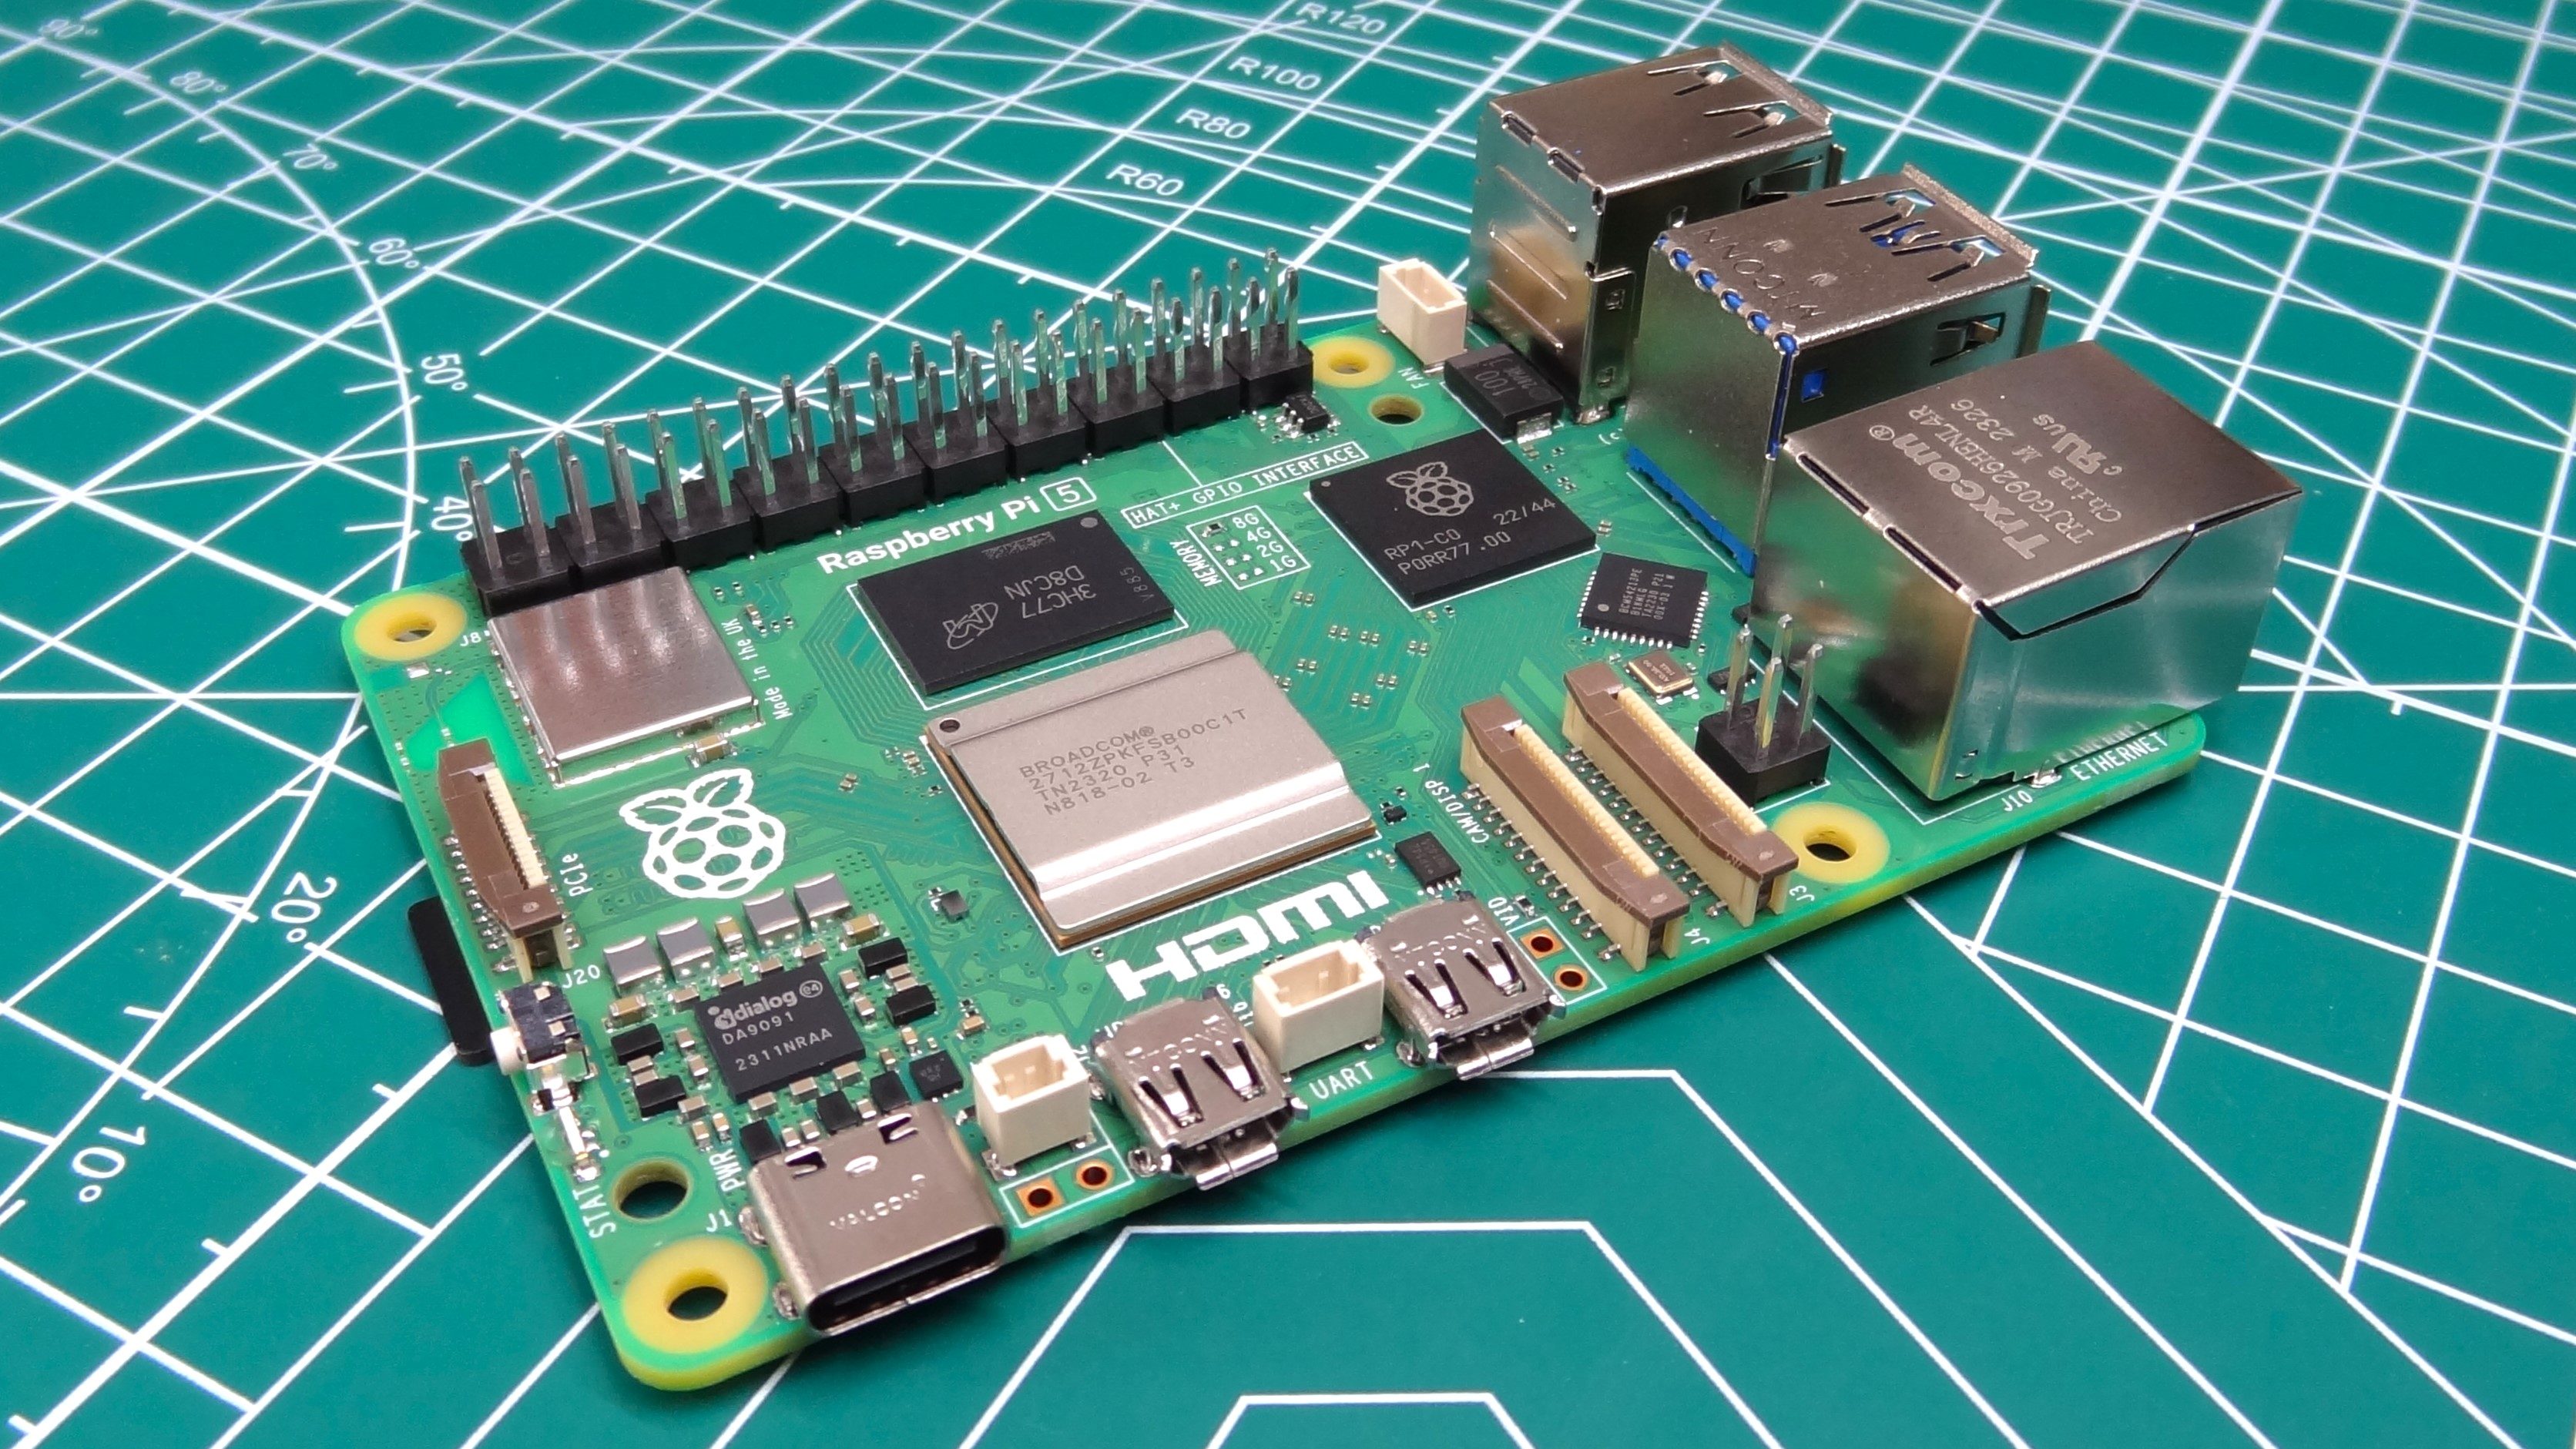
\includegraphics[width=\textwidth]{raspberry_pi_5}
                \caption{Raspberry Pi 5}
            \end{subfigure}
\hfill
            \begin{subfigure}{0.3\textwidth}
                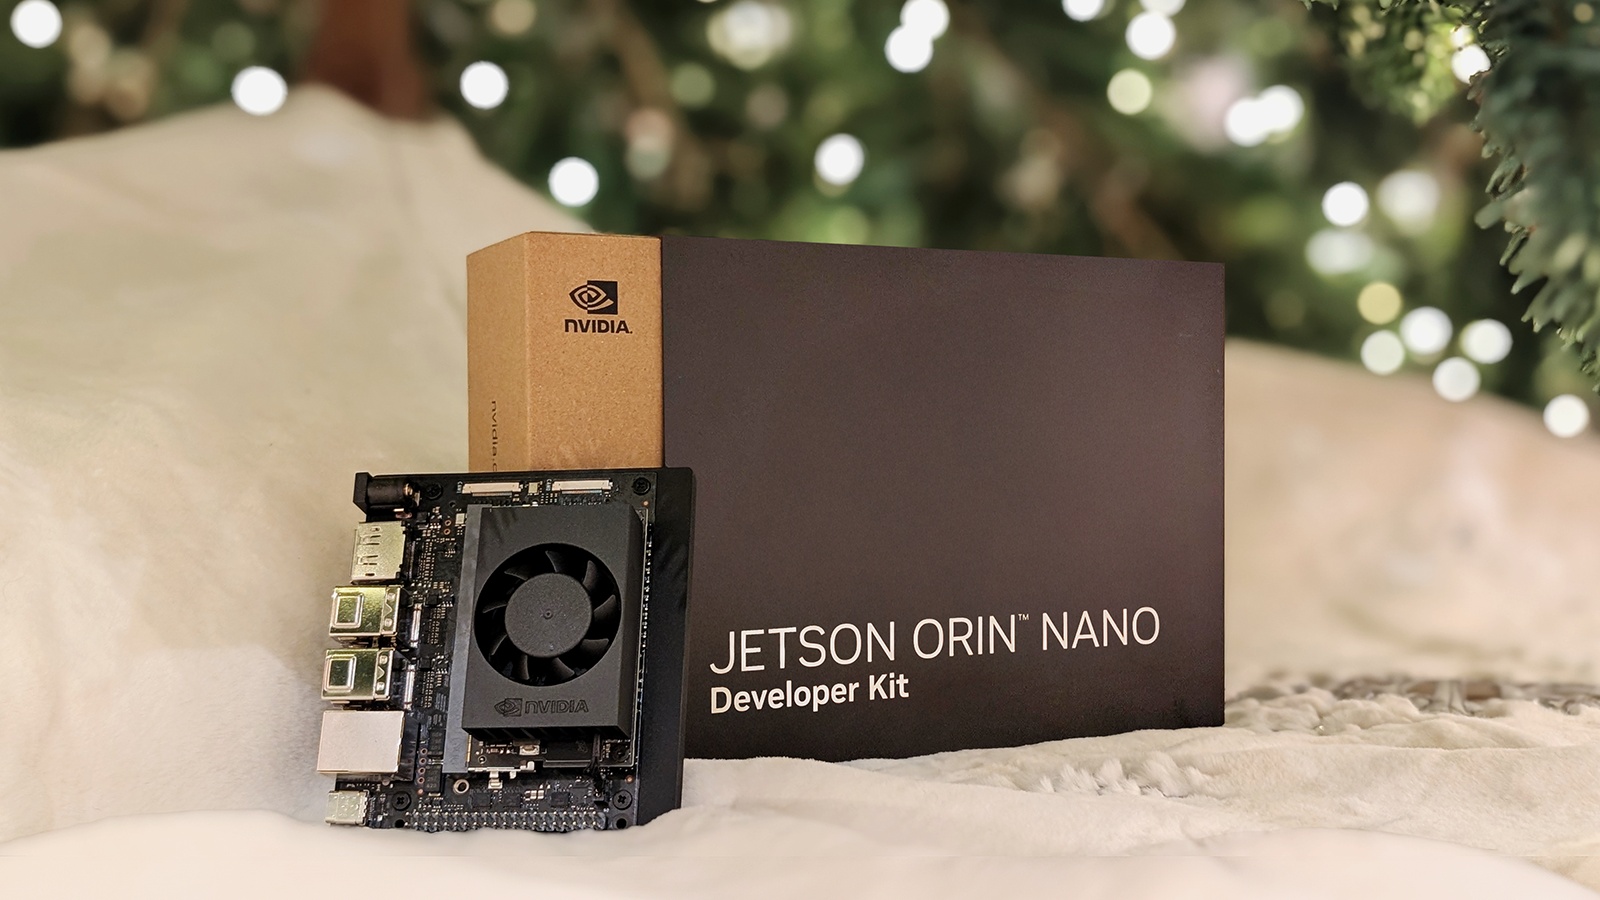
\includegraphics[width=\textwidth]{jetson_orin_nano}
                \caption{Jetson Orin Nano}
            \end{subfigure}
\hfill
            \begin{subfigure}{0.3\textwidth}
                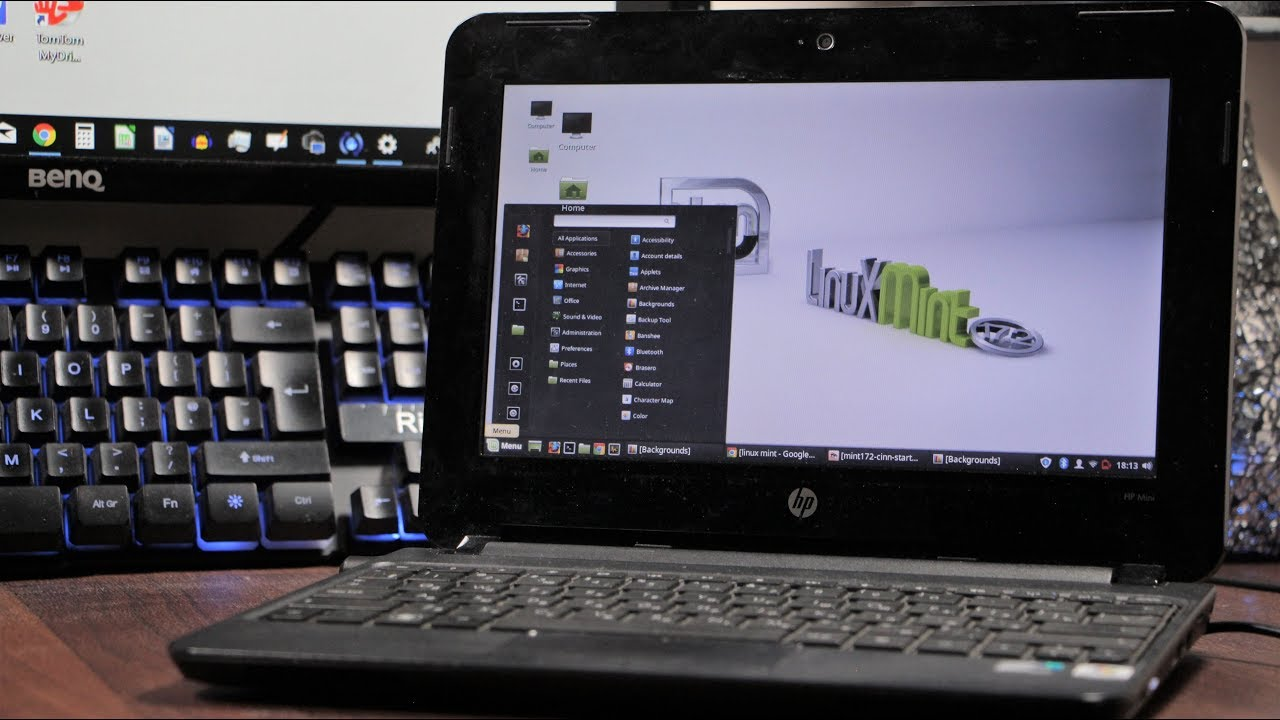
\includegraphics[width=\textwidth]{old_laptop_server}
                \caption{Old laptop or desktop}
            \end{subfigure}
        \end{center}
    \end{figure}

    \begin{itemize}
        \item Raspberry Pi 5: small, 3-15 W, runs full Linux, huge community
        \item NVIDIA Jetson: small GPU on a Pi-sized board, for heavier on-device AI
        \item Old laptop/desktop: more RAM, free, laptop has a built-in UPS
        \item Or build a home server from PC parts for any budget
    \end{itemize}
\note{
}
\end{frame}


\begin{frame}{Getting the OS on it}
    Unlike a cloud VM, our device does not arrive booted.
    Each platform has an official imager.

    \begin{itemize}
        \item Raspberry Pi: \emphasis{Raspberry Pi Imager} writes a preconfigured SD card
        \item Jetson: \emphasis{JetPack SDK} ships an image with GPU drivers
        \item Old x86 laptop or desktop: Ubuntu Server on a USB stick made with balenaEtcher
    \end{itemize}

    \vspace{0.5em}
    Once the OS is up, our device is at the same starting line as the cloud VM.
    The rest of the workflow is identical.
\note{
}
\end{frame}


\begin{frame}{The small caveat from B.2}
    In Module B.2 we said a container image runs anywhere a runtime is installed.
    We glossed over a small caveat: an image is built for a specific CPU architecture, and only runs on a machine with the same CPU architecture.

    \begin{itemize}
        \item \emphasis{x86-64} (\texttt{amd64}): almost every desktop, laptop, and most cloud VMs
        \item \emphasis{ARM64} (\texttt{aarch64}): smartphones, Raspberry Pi, Jetson, Apple Silicon Macs, and some cloud VMs
        \item \emphasis{RISC-V}: newer, open-source, mostly microcontrollers today but growing fast
    \end{itemize}

    \vspace{0.5em}
    An image built for x86-64 will not run on a Raspberry Pi with an ARM64 CPU.
\note{
}
\end{frame}


\begin{frame}{Multi-architecture images}
    Most popular images on Docker Hub publish builds for several architectures.

    \begin{figure}[htpb]
        \begin{center}
            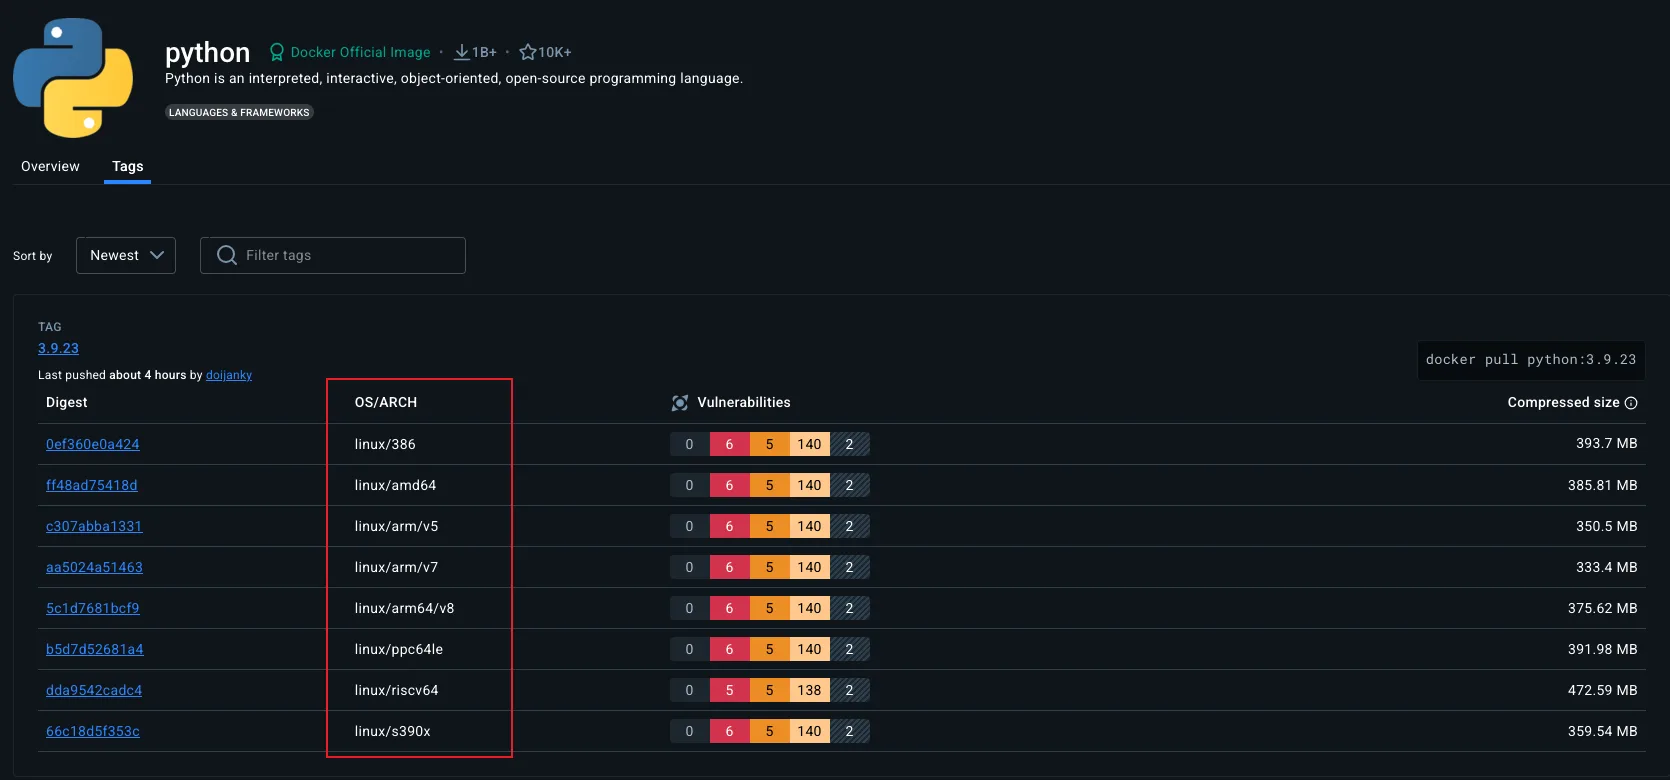
\includegraphics[width=0.55\textwidth]{docker-hub-platforms}
        \end{center}
    \end{figure}

    \texttt{docker pull python:3.13} on a Pi pulls the ARM64 variant automatically.
    No extra flags needed.
\note{
}
\end{frame}


\begin{frame}[fragile]{Building for multiple architectures}
    Two options for our own images.

    \begin{block}{Simple: build on the target}
        SSH into the Pi, copy the project, run \texttt{docker build}.
        Image comes out ARM64.
    \end{block}

    \begin{block}{Sophisticated: Buildx, one machine, many archs}
        \begin{minted}{bash}
docker buildx build --platform linux/amd64,linux/arm64 \
    -t yourusername/my-ai-server:1.0 --push .
        \end{minted}
        Builds the same Dockerfile for both, emulating the non-host architecture.
        Pushes both variants under the same tag.
    \end{block}
\note{
}
\end{frame}



\section{Getting Past NAT}

\begin{frame}{The cloud VM had a public IP}
    For a cloud VM, anyone on the internet could type that IP into their browser and reach our server, since a cloud VM is usually assigned a public IP address.
    Our edge or self-hosted device, which sits on a home or office network, usually does not enjoy this.

    \begin{figure}[htpb]
        \begin{center}
            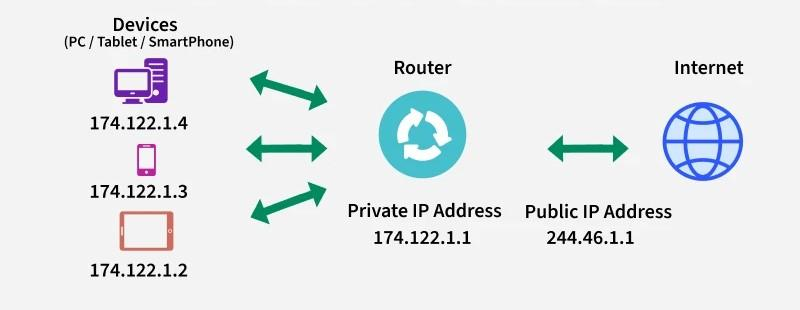
\includegraphics[width=0.42\textwidth]{nat_diagram}
        \end{center}
    \end{figure}
\note{
}
\end{frame}


\begin{frame}{How NAT hides us}
\textbf{Network Address Translation (NAT)} is the trick that lets every device on a home network share a single public IP.

    \begin{itemize}
        \item The router has a public IP from the ISP, shared by every device behind it
        \item The router gives each connected device a private IP like \texttt{192.168.1.42}
        \item Outgoing requests: router rewrites the source, remembers the connection in a table
        \item Incoming requests: router has no idea where to send the request, so it drops it
    \end{itemize}

    Outgoing connections work fine. Incoming connections do not.
    An AI API server has to accept incoming.
\note{
}
\end{frame}


\begin{frame}{CGNAT makes it worse}
With \textbf{Carrier-grade NAT (CGNAT)}, the ISP itself does another layer of NAT in front of many customers.
    Even the public IP our router thinks it has is shared with other users.

    \begin{itemize}
        \item Almost always on mobile networks
        \item Also increasingly common on fiber internet as IPv4 addresses run out
    \end{itemize}

    \vspace{0.5em}
    Behind CGNAT, no amount of router configuration on our side will help.
\note{
}
\end{frame}


\begin{frame}{Three paths through NAT}
    \begin{enumerate}
\item \textbf{Port forwarding} plus \textbf{dynamic DNS}, if we have a real public IP
\item Cloud VM as a reverse proxy through a \textbf{VPN tunnel}
        \item Managed tunnel services
    \end{enumerate}
\note{
}
\end{frame}


\begin{frame}{Port forwarding and DDNS}
    If our ISP gives us a real public IP (no CGNAT):

    \begin{block}{Port forwarding on the router}
        Tell the router that incoming traffic on certain ports should go to a certain device.
        Most routers have a settings page for this.
    \end{block}

    \begin{block}{Dynamic DNS}
        Home IPs, even when public, are usually dynamic. They change every few weeks.
        A small daemon on the device tells a DDNS provider the current IP, and the provider updates the DNS record.
    \end{block}

    Static public IP from the ISP, as a paid add-on, removes the need for DDNS. Availability varies.
\note{
}
\end{frame}


\begin{frame}{Cloud VM as a reverse proxy}
    If CGNAT blocks the direct route, borrow a public IP by renting a small cloud VM.
    Same reverse proxy from B.4, just pointing through a tunnel to our edge device.

    \begin{figure}[htpb]
        \begin{center}
            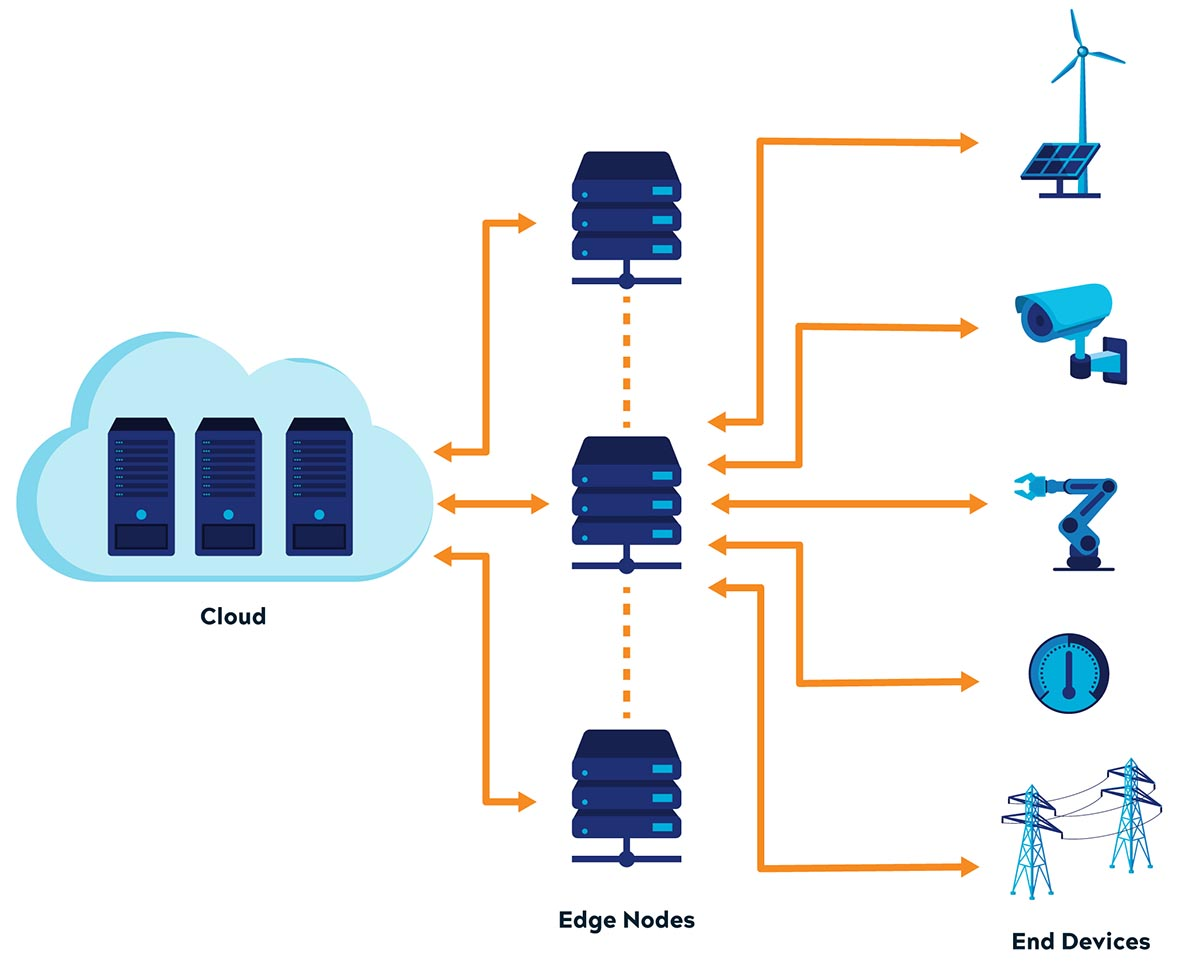
\includegraphics[width=0.32\textwidth]{edge_topology}
        \end{center}
    \end{figure}

    Edge device opens an outgoing connection to the cloud VM through a VPN tunnel (usually \textbf{WireGuard}).
    Cloud VM's Nginx forwards through the tunnel instead of to a local container.
\note{
}
\end{frame}


\begin{frame}[fragile]{Pointing Nginx through the tunnel}
    Assume the cloud VM is \texttt{10.0.0.1} and the edge device is \texttt{10.0.0.2} on the WireGuard tunnel.

    \begin{minted}{nginx}
location / {
    proxy_pass http://10.0.0.2:8000;
    proxy_set_header Host $host;
    proxy_set_header X-Real-IP $remote_addr;
    proxy_set_header X-Forwarded-For $proxy_add_x_forwarded_for;
    proxy_set_header X-Forwarded-Proto $scheme;
}
    \end{minted}

    Only change from B.4: \texttt{proxy\_pass} points to the tunnel address.
\note{
}
\end{frame}


\begin{frame}{IPv6, briefly}
    Many ISPs now provide IPv6 alongside IPv4.
    IPv6 has a large enough address space that every device can have its own globally routable address. No NAT.

    \vspace{0.5em}
    If both our device and the client device have IPv6, publish an \texttt{AAAA} DNS record pointing to the device's IPv6 address.
    Connections work without any tunneling.

    \vspace{0.5em}
    Catch: not all internet users have IPv6 yet, so we usually still need an IPv4 path through one of the options above.
\note{
}
\end{frame}



\section{Backups}

\begin{frame}{Backups are now our job}
    On a cloud VM we usually get a baseline of reliability for free.
    Most providers replicate the underlying disks, swap failed hardware, and let us snapshot the entire VM with a click of a button.
    None of that is true on our own hardware.

    \begin{itemize}
        \item SD cards commonly have a high failure rate after a few years of heavy writes
        \item Hard drives will die eventually
        \item Laptops often get spilled on
    \end{itemize}

    If we are going to put real data on a self-hosted system, backups are part of our job.
\note{
}
\end{frame}


\begin{frame}{The 3-2-1 rule}
    \begin{block}{Keep}
        \begin{itemize}
            \item At least 3 copies of the data
            \item On 2 different storage media
            \item With 1 copy stored offsite
        \end{itemize}
    \end{block}

    \begin{block}{Why}
        \begin{itemize}
            \item If a single disk dies and takes one copy, the other two survive
            \item If a fire or theft takes everything in the building, the offsite copy survives
        \end{itemize}
    \end{block}

    Applied properly, the chance of losing data drops to a very small number.
\note{
}
\end{frame}



\section{Exercise}

\begin{frame}{Self-host your AI server}
    Take the image from Module B.3. Host it on hardware you own.
    Make it publicly accessible.
    The cloud VM from B.4 becomes the reverse proxy.

    \begin{block}{Outline}
        \begin{enumerate}
            \item Use your daily computer as the edge device, or use a "real" edge device if available
            \item Get it online, install Docker, run the container. Verify the server's reachability from another local machine
            \item Set up a VPN tunnel between the B.4 cloud VM and the device and point the Nginx proxy on the cloud VM to the edge device
            \item From outside your home network, point the A.2 client at the public URL
        \end{enumerate}
    \end{block}
\note{
}
\end{frame}


\begin{frame}{Extensions}
    \begin{enumerate}
        \item Set up periodic backups of the SQLite database. Simulate a file loss and restore from the backup
        \item Compare response time of the self-hosted server vs the cloud-VM version. Depending on your hardware and home network, self-hosted may be faster despite the cloud VM having professional infrastructure
    \end{enumerate}
\note{
}
\end{frame}


\begin{frame}{What you should walk away with}
    By the end of the exercise, you should be able to:
    \begin{enumerate}
        \item Understand edge computing and self-hosting, and when to choose them
        \item Deploy the same container onto hardware you own
        \item Make a device behind NAT reachable, and keep its data backed up
    \end{enumerate}

    \vspace{0.5em}
    This closes Part B. You can now take an AI system from your own laptop to specialized hardware, containers, the cloud, and the edge.
\note{
}
\end{frame}



\appendix

\begin{frame}[plain,noframenumbering]
\begin{center}
{\large Thank you!}
\vspace{1cm}
\\[0.5em]
{\small \faEnvelope\ \href{mailto:lyan@cs.aau.dk}{lyan@cs.aau.dk} \\
\faGlobe\ \href{https://www.yanlincs.com}{www.yanlincs.com}}
\end{center}
\note{
}
\end{frame}

\end{document}
